%\documentclass{proc}  % 2-column format
\documentclass[12pt]{paper}
%\documentclass{ntmanuscript}
%\documentclass[review]{elsarticle}
\usepackage{mathptmx} % Nearly Times New Roman
\usepackage[acronym,toc]{glossaries}
\newacronym{MIT}{MIT}{the Massachusettes Institute of Technology}
\newacronym{UW}{UW}{University of Wisconsin}
\newacronym{US}{US}{United States}
\newacronym{HEU}{HEU}{highly enriched uranium}
\newacronym{LEU}{LEU}{low enriched uranium}
\newacronym{U}{U}{uranium}
\newacronym{SWU}{SWU}{separative work unit}
\newacronym{CNERG}{CNERG}{Computational Nuclear Engineering Research Group}
\newacronym{DRE}{DRE}{dynamic resource exchange}
\newacronym{UOX}{UOX}{uranium oxide}
\newacronym{MOX}{MOX}{mixed oxide}


\newacronym{IAEA}{IAEA}{International Atomic Energy Agency}
\newacronym{SNF}{SNF}{spent nuclear fuel}
\newacronym{HLW}{HLW}{high level waste}
\newacronym{FEHM}{FEHM}{Finite Element Heat and Mass Transfer}
\newacronym{DOE}{DOE}{Department of Energy}
\newacronym{GENIUSv1}{GENIUS}{Global Evaluation of Nuclear Infrastructure 
Utilization Scenarios, Version 1}
\newacronym{GENIUSv2}{GENIUS}{Global Evaluation of Nuclear Infrastructure Utilization Scenarios, Version 2}
\newacronym{GDSM}{GDSM}{Generic Disposal System Model}
\newacronym{GDSE}{GDSE}{Generic Disposal Sytem Environment}
\newacronym{GPAM}{GPAM}{Generic Performance Asessment Model}
\newacronym{FEPs}{FEPs}{Features, Events, and Processes}
\newacronym{EBS}{EBS}{Engineered Barrier System}
\newacronym{EDZ}{EDZ}{Excavation Disturbed Zone}
\newacronym{YMR}{YMR}{Yucca Mountain Repository Site}
\newacronym{EPA}{EPA}{Environmental Protection Agency}
\newacronym{PEI}{PEI}{Peak Environmental Impact}
\newacronym{VISION}{VISION}{the Verifiable Fuel Cycle Simulation Model}
\newacronym{NUWASTE}{NUWASTE}{Nuclear Waste Assessment System for Technical Evaluation}
\newacronym{NWTRB}{NWTRB}{Nuclear Waste Technical Review Board}
\newacronym{OCRWM}{OCRWM}{Office of Civillian Radioactive Waste Management}
\newacronym{UFD}{UFD}{Used Fuel Disposition}
\newacronym{DYMOND}{DYMOND}{Dynamic Model of Nuclear Development }
\newacronym{DANESS}{DANESS}{Dynamic Analysis of Nuclear Energy System Strategies}
\newacronym{CAFCA}{CAFCA}{ Code for Advanced Fuel Cycles Assessment }
\newacronym{ORION}{ORION}{O..}
\newacronym{NFCSim}{NFCSim}{Nuclear Fuel Cycle Simulator}
\newacronym{COSI}{COSI}{Commelini-Sicard}
\newacronym{FCT}{FCT}{Fuel Cycle Technology}
\newacronym{SWF}{SWF}{Separations and Waste Forms}
\newacronym{FCO}{FCO}{Fuel Cycle Options}
\newacronym{RDD}{RD\&D}{Research Development and Design}
\newacronym{WIPP}{WIPP}{Waste Isolation Pilot Plant}
\newacronym{ANDRA}{ANDRA}{Agence Nationale pour la gestion des D\'echets RAdioactifs, the French National Agency for Radioactive Waste Management}
\newacronym{TSM}{TSM}{Total System Model}
\newacronym{LANL}{LANL}{Los Alamos National Laboratory}
\newacronym{INL}{INL}{Idaho National Laboratory}
\newacronym{ANL}{ANL}{Argonne National Laboratory}
\newacronym{SNL}{SNL}{Sandia National Laboratory}
\newacronym{LBNL}{LBNL}{Lawrence Berkeley National Laboratory}
\newacronym{LLNL}{LLNL}{Lawrence Livermore National Laboratory}
\newacronym{NAGRA}{NAGRA}{National Cooperative for the Disposal of Radioactive Waste}
\newacronym{CUBIT}{CUBIT}{CUBIT Geometry and Mesh Generation Toolkit}
\newacronym{CSNF}{CSNF}{Commercial Spent Nuclear Fuel}
\newacronym{DSNF}{DSNF}{DOE Spent Nuclear Fuel}
\newacronym{MTHM}{MTHM}{Metric Ton of Heavy Metal}
\newacronym{HTGR}{HTGR}{High Temperature Gas Reactor}
\newacronym{TRISO}{TRISO}{Tristructural Isotropic}
\newacronym{MA}{MA}{Minor Actinide}
\newacronym{CEA}{CEA}{Commissariat a l'Energie Atomique et aux Energies Alternatives}
\newacronym{SKB}{SKB}{Svensk Karnbranslehantering AB}
\newacronym{SINDAG}{SINDA{\textbackslash}G}{Systems Improved Numerical Differencing Analyzer $\backslash$ Gaski}
\newacronym{STC}{STC}{Specific Temperature Change}
\newacronym{LDRD}{LDRD}{Laboratory Directed Research and Development}
\newacronym{LCOE}{LCOE}{Levelized Cost of Electricity}
\newacronym{ABM}{ABM}{Agent-Based Modeling}
\newacronym{COTS}{COTS}{Commercial, Off-The-Shelf}
\newacronym{API}{API}{Application Programming Interface}
\newacronym{RIF}{RIF}{Region-Institution-Facility}
\newacronym{GUI}{GUI}{Graphical User Interface}
\newacronym{HPC}{HPC}{High-Performace Computing}
\newacronym{HTC}{HTC}{High-Throughput Computing}
\newacronym{UML}{UML}{Unified Modeling Language}
\newacronym{DAG}{DAG}{Directed Acyclic Graph}
\newacronym{XML}{XML}{Extensible Markup Language}
\newacronym{RNG}{RelaxNG}{REgular LAnguage for XML Next Generation}
\newacronym{JSON}{JSON}{JavaScript Object Notation}
\newacronym{SQL}{SQL}{Structured Query Language}
\newacronym{SQLite}{SQLite}{Structured Query Lite}
\newacronym{HDF5}{HDF5}{Hierarchical Data Format version 5}
\newacronym{CSV}{CSV}{Comma-Separated Value}
\newacronym{VL}{VL}{Variable Length}
\newacronym{SHA1}{SHA1}{Secure Hash Algorithm 1}
\newacronym{YAML}{YAML}{Yet-Another Markup Language}
\newacronym{POSIX}{POSIX}{Portable Operating System Interface}
%\newacronym{<++>}{<++>}{<++>}
%\newacronym{<++>}{<++>}{<++>}
%\newacronym{<++>}{<++>}{<++>}
%\newacronym{<++>}{<++>}{<++>}

%\makeglossaries
%%%%%%%%%%%%%%%%%%%%%%%%%%%%%%%%%%%

\usepackage{color}
\usepackage{subcaption}
\usepackage{graphicx}
\usepackage{booktabs} % nice rules for tables
\usepackage{microtype} % if using PDF
\usepackage{xspace}
\usepackage{listings}
\usepackage{textcomp}
%\usepackage{ulem}

% Page length commands go here in the preamble
\setlength{\oddsidemargin}{-0.25in} % Left margin of 1 in + 0 in = 1 in
\setlength{\textwidth}{7in}   % Right margin of 8.5 in - 1 in - 6.5 in = 1 in
\setlength{\topmargin}{-.75in}  % Top margin of 2 in -0.75 in = 1 in
\setlength{\textheight}{9.2in}  % Lower margin of 11 in - 9 in - 1 in = 1 in



\definecolor{listinggray}{gray}{0.9}
\definecolor{lbcolor}{rgb}{0.9,0.9,0.9}
\lstset{
    %backgroundcolor=\color{lbcolor},
    language={C++},
    tabsize=4,
    rulecolor=\color{black},
    upquote=true,
    aboveskip={1.5\baselineskip},
    belowskip={1.5\baselineskip},
    columns=fixed,
    extendedchars=true,
    breaklines=true,
    prebreak=\raisebox{0ex}[0ex][0ex]{\ensuremath{\hookleftarrow}},
    frame=single,
    showtabs=false,
    showspaces=false,
    showstringspaces=false,
    basicstyle=\scriptsize\ttfamily\color{green!40!black},
    keywordstyle=\color[rgb]{0,0,1.0},
    commentstyle=\color[rgb]{0.133,0.545,0.133},
    stringstyle=\color[rgb]{0.627,0.126,0.941},
    numberstyle=\color[rgb]{0,1,0},
    identifierstyle=\color{black},
    captionpos=t,
}

\newcommand{\code}[1]{\lstinline[basicstyle=\ttfamily\color{green!40!black}]|#1|}
\newcommand{\units}[1] {\:\text{#1}}%
\newcommand{\SN}{S$_N$}
\newcommand{\cyclus}{\textsc{Cyclus}\xspace}
\newcommand{\Cyclus}{\cyclus}
\newcommand{\citeme}{\textcolor{red}{CITE}\xspace}
\newcommand{\TODO}[1] {{\color{red}\textbf{TODO: #1}}}%

\newcommand{\comment}[1]{{\color{green}\textbf{#1}}}

%%%%%%%%%%%%%%%%%%%%%%%%%%%%%%%%%%%
\begin{document}


%\begin{frontmatter}
\title{State-Level Decision-Making In Cyclus to Assess Multilateral Enrichment}

% Authors. Separated by commas
\author{
  Meghan B. McGarry$^1$,
  Chris Hoffman$^1$,
  Drew Buys$^1$,
  Baptiste Mouginot$^1$,
  Paul P.H. Wilson$^1$}


\date{}
% Institutes of the authors
\institution{$^1$Department of Nuclear Engineering and Engineering Physics,
University of Wisconsin-Madison}
%\\$^2$Sandia National Laboratories}
% Information concerning the person submitting the manuscript
%\submitter{Meghan B. McGarry}
%\submitteraddress{1500 Engineering Drive, Madison, WI, USA}
%\submitteremail{mbmcgarry@wisc.edu}

% No more than three keywords, though each can be a phrase
%\keywords{fuel cycle, simulatiom, non-proliferation}
\maketitle

% I. Motivation
% x   -  Identify Factors that motivate
% x  II. Benchmark model against historical data:
% x A. Develop historical database
% x   - What sources?
% x   - What model to convert to 10pt scale?
% x        - Conflict
% x B. Determine relative weighting of factors
% x   - Calculate values for historical database
% x   - PCA to determine relative weights
% ** C. Table of State Score Results
% III. Develop forward model 
%   - From score to a likelihood, using historical data
% IV. Limitations of model
%   - small dataset
%   - threshold value for proliferation
%   - no good model for scientific network
% V. Future work
%   - Apply to case study (JCPOA?)
% VI Appendix of factor conversions

\begin{abstract}

 Proposed treaties and agreements that aim to reduce the spread of nuclear weapons are often stalled by skepticism regarding their efficacy. For example, the concept of multilateral enrichment, in which multiple states co-own and operate an enrichment facility, has the potential to reduce the spread of enrichment technology. However, detractors point to the improved international networking opportunities inherent in multinational organizations as a risk factor for increased proliferation. A framework to compare the relative risk between a multilateral enrichment paradigm and the status quo, on a regional scale, can help inform the discussion and potentially identify ways to reduce global risk of nuclear proliferation. As part of the Consortium for Verification Technology, the Cyclus fuel cycle simulator is being used as a test-bed for the development of such new technologies and approaches to treaty verification. Cyclus is a systems-level nuclear fuel cycle simulator that models the interactions between actors in the nuclear arena. While designed to track the flow of nuclear material between facilities, Cyclus also incorporates an innovative Facility-Institution-Region hierarchy that can capture the dynamics of state-level interactions. Drawing on social science literature to identify factors that motivate states to pursue weapons programs, we have developed a regional proliferation model that captures causes and effects of state-level nuclear weapons proliferation. The model identifies eight key factors that influence a state’s decision to pursue nuclear weapons. These factors include motivations internal to the state, such as military spending and governing structure, as well as interactive factors such as conflict between states. Historical data is used to identify the relative importance of these factors and translate them into a likelihood of pursuing a weapon. The model also provides a feedback mechanism such that acquisition of a nuclear weapon by one state influences the decision-making of the other states. This model will be used to assess the effectiveness of policy approaches, such as multilateralization of the fuel cycle, that seek to reduce the regional risk of proliferation over time.

\end{abstract}


%\end{frontmatter}


\section{Motivation}
\label{s_motive}

In the 70 years since nuclear bombs were dropped on Hiroshima and Nagasaki, the knowledge and technology required to make these weapons has proliferated around the globe. There are now nine states that have developed their own nuclear weapons, as well as many others who have the capability to do so\cite{feiveson_unmaking_2014}.  Moreover, this knowledge will continue to spread as climate change change further tilts the scales such that the benefits of nuclear power outweigh the risks \cite{mooney_why_2014}.  China is already investing heavily in nuclear power, planning to triple its generating capacity from 19GWe to 58GWe by 2020  \cite{_china_2014}.  As climate change increasingly dominates discussions of national security, the perception of the risks inherent to nuclear energy is decreasing and states are embracing nuclear energy as a reliable large-scale source of carbon-neutral energy.  However, the expansion of nuclear power increases concerns with respect to nuclear security, because the same technologies used to produce nuclear fuel can also be exploited in the pursuit of nuclear weapons.


\subsection{Sensitive Parts of the Nuclear Fuel Cycle}

Two nuclear technologies are of of particular concern for proliferation, uranium enrichment and plutonium reprocessing.  Urnaium enrichment is required for the once-through fuel cycles that are dominant around the world today, and used exclusively in the US.  A once-through fuel cycle includes a source of natural uranium such as a mine, and is comprised of non-fissile 99.3\% $^{238}U$ and only 0.7\% fissile $^{235}U$. Concentrations of 4-20\% fissile $^{235}U$ are required to fuel a nuclear reactor. Enrichment facilities are used to increase the concentration of $^{235}U$ to the desired amount.  Fuel is then burned in a nuclear reactor and the remaining material, which includes the original $^{238}U$, short- and long-lived fission products, as well as \~1\% $^{239}Pu$ and $^{240}Pu$, is then stored as waste.  The enrichment facility is notable because it can be used to increase the concentration of $^{235}U$ up to the 80-90\% required to make a nuclear weapon\cite{_military_2014}.

Several countries are developing nuclear reactors that can accomodate recycled fuel \cite{_processing_2015}.  Recycled fuel is plutonium-based rather than uranium-based, and is made by separating the components of spent uranium fuel and increasing the concentration of fissile $^{239}Pu$ up to 80\%.  This material can then be used as fuel or blended with uranium to make \gls{MOX}.  As with the enrichment process however, separations facilities can increase the concentration beyone that required for fuel to generate \gls{WGP} (up to 93\% $^{239}Pu$).  However, fuel cycles with the capability to burn \gls{MOX} fuel are advangteous because \gls{WGP} from decommissioned nuclear weapons can be blended into \gls{MOX}, which reduces the amount of \gls{SNM} that must be safeguarded.  In part due to the large stockpile of \gls{WGP} in the \gls{US}, reprocessessing has been considered at several times over the past half-century.  However, a host of political, economic, environmental and strategic concerns have cpushed the issue of reprocessing out of the technical realm and it has become a contentious political topic, and currently the \gls{US} is pursuing only basic science research in this field \cite{rossin_policy_????, _adieu_2009}.
 
\subsection{Use of Treaties to Minimize Proliferation}

While it has not proven possible to prevent the spread of nuclear knowledge entirely, international treaties have been used in an attempt to control it.  The \gls{NPT}, which has been signed by 190 states including the original 5 nuclear weapons states, has codified a set of rules and norms for allowing the peaceful pursuit of nuclear energy\cite{_treaty_????}.  The \gls{NPT} created an organization called \gls{IAEA}, whose role is to verify compliance with the treaty by periodically inspecting facilities related to nuclear technology.  Other notable treaties include \gls{CTBT}, which placed a moratorium on testing nuclear weapons, and the \gls{START} in which the \gls{US} and Russia agreed on nuclear arms reductions.

These treaties seek to have done much to prevent the spread of nuclear weapons, but they do not address the production capabilities of states that already posess nuclear weapons.  A potential \gls{FMCT} would place limits on the amount of \gls{SNM} each weapons state could stockpile, possibly including current stockpiles in addition to future production.  However, a major unresolved issue is the difficulty of developing verification techniques that can reliably confirm that nuclear material is not being produced \cite{_fissile_2013}.  Furthermore, making measurements of nuclear material for treaty verification is itself a sensitive issue, as even collecting the spectra of a material to confirm its authenticity can potentially expose sensitive information\cite{glaser_zero_2014}. Particularly if non-weapons states are to contribute to treaty verification, it is important to prevent the further dissemination of nuclear knowledge.

\begin{figure}%[htbp!]
\begin{center}
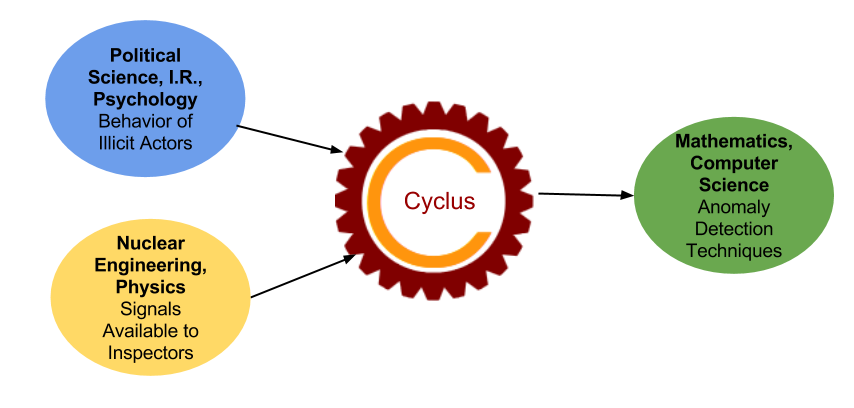
\includegraphics[natwidth=162bp,natheight=227bp, scale=0.5]{./figs/cyclus_interdiscipline.png}
\end{center}
\caption{The \Cyclus nuclear fuel cycle simulator provides a testbed to integrate innovations in treaty verification across many disciplines.}
\label{fig:cyclus_diagram}
\end{figure}

An effective treaty verification regime must synthesize knowledge from the realmns of political science, international relations, nuclear physics and engineering, and even behavioral psychology.  A nuclear fuel cycle simulator provides a framework in which to integrate these disparate components into an effective strategy.  As shown in Figure \ref{fig:cyclus_diagram}, a fuel cycle simulator can combine the technical specifications of innovative detection modalities, signal processing techniques, and models of the social-behavioral interactions between actors to provide insights into proposed verification approaches.  At a systems level, a fuel cycle simulator can be used to frame test scenarios as responses to stimuli. That is, even if not all of the specific details are available, simulations can incorporate response behaviors to illucidate the strengths and weaknesses of various verification strategies.



\section{Factors That Correlate to Pursuit of Nuclear Weapons}
\label{s_factors}

Social science literature has suggested that a variety of political and technical factors that may motivate a state to pursue nuclear weapons\cite{bell_questioning_2013, singh_correlates_2004, montgomery_perils_2009, li_model-based_2010, hymans_achieving_2012}. Political factors include: degree to which governing structure is authoritarian versus democratic, level of military spending, degree to which state is isolated militarily, and level of conflict with other states. Technical factors include: degree to which the state's scientific expertise is integrated into the international community, nuclear reactor experience, indigenous reserves of natural uraniaum, and the ability to enrich uranium.

We have compiled a database of information that quantifies each of these eight factors for states at important historical points, publically available on github\footnote{https://github.com/CNERG/historical\_prolif/blob/master/clean\_raw\_data.csv}, along with documentation on source data and assumptions\cite{hist_prolif}. The set includes 43 unique states that have historically had either nuclear energy or weapons technology.  The 24 states that have never pursued weapons have data compiled for 2015. The 19 states that have pursued weapons at some point in the past have data for the year in which they pursued as well as the year in which they acquired a weapon, if applicable. Pursuit and acquisition dates are coded from \emph{Singh and Way}. The pursuit date is defined as the first year in which a significant decision to pursue nuclear weapons was made such as a political decision by cabinet-level officials, movement toward weaponization, or development of single-use, dedicated technology.  Acquire date indicates the year in which either the first explosion of a nuclear device occurred or the complete assembly of a weapon since not all countries tested their nuclear weapons.

\begin{table}
\centering
\begin{tabular}{|c|c|}
\hline
\textbf{Factor}        & \textbf{Source Database} \\
\hline
Authoritarian            & Center for Systemic Peace \\
                          & Polity IV Annual Time-Series, 1800-2015\cite{polity_scores}\\
\hline
Conflict & Uppsala Conflict Data Program \\
         & Armed Conflict Dataset\cite{conflict_ref} \\
\hline
Enrichment/Reprocessing   & Nuclear Latency Dataset \cite{latency_ref} \\
\hline
Military Isolation & Rice University \\
& The Alliance Treaty Obligations and Provision Project\cite{mil_iso}\\
\hline
Military Spending & Stockholm International Peace Research Institute \\
    & Military Expenditure Database 1949-2015\cite{mil_sp} \\
\hline
Nuclear Reactors           &  IAEA Power Reactor Database \cite{power_react}\\

                         & IAEA Research Reactor Database \cite{research_react}\\
\hline
Scientific Network     & Authors' Expert Opinion\footnote{Considers GDP, opportunities for scientists to study abroad, nuclear infrastructure, technical human capital} \\
\hline
Uranium Reserves  &    OECD Uranium: Resources, Production and Demand \cite{noauthor_uranium_2014} \\
\hline
\end{tabular}
\caption{Source data for each factor contributing to pursuit of nuclear weapons addressed in this paper.}
\label{tab:factor_sources}
\end{table}

\subsection{Pursuit Score}\label{s_pe}
The source used to define each factor has been taken from social science literature and is listed in Table \ref{tab:factor_sources} The raw data for each attribute has been normalized on a 1-10 scale so that all factors can be compared directly, as described in Table \ref{tab:factor_conversions}. Conflict is shown separately in Table \ref{tab:conflict}. Conflict has been defined for a given state by using the \emph{Uppsala database} to identify up to three significant state-pair relationships based on the state's conflicts during that year (the dataset was limited to three as a starting point, but could be further expanded).   Each of these relationships is coded as enemy, neutral, or ally.  Each of the two states in the pair is also identified as being a \gls{NNWS}, known to be pursuing weapons, or a \gls{NWS}.  The combination of weapons status and relationship status is combined to provide a conflict score for each pair. The net conflict factor is the average of all the state's paired conflict scores. We consider that the pursuit phase is the most destabilizing, and have incorporated considerations such as nuclear umbrellas \TODO{cite},  preventative war, increased low-level conflict between weapons states \cite{geller_nuclear_1990, fuhrmann_targeting_2010, bell_questioning_2013-1}.

%\begin{landscape}
\begin{table}
\centering
\begin{tabular}{|c|c|c|c|c|c|c|c|c|c|}
\hline
\textbf{Factor}      & \textbf{Auth}          & \textbf{Enrich/}      & \multicolumn{2}{c|}{\textbf{Military Iso.}}          & \textbf{Mil. Spend} &  \textbf{Reactors}  & \textbf{Sci.} & \textbf{Uran.} \\
\textbf{Score}  &                        &  \textbf{Repro.}   & \multicolumn{2}{c|}{$10 - (A_{NNWS}+A_{NWS})$}  & \textbf{(\%GDP)}    &   (Power+Research) & \textbf{Net.} &  \textbf{Res} \\
\cline{4-5}
 (FS)           &                         &                       &  NNWS                 & NWS               &                    & $10 - R_{all}$&               &              \\


\hline
\textbf{0}      &  0                     &  0                   &  --                        &  --                     &  --                 &   0                   &    --         &  0           \\   
\textbf{1}      &  1                     &  --                  &  1-2                       &  --                     &  $<$ 1              &   1-3 planned         &    --         &  --          \\
\textbf{2}      &  2                     &  --                  &  3-4                       &  --                     &  [1, 2)             &   4+ planned          &    --         &  --          \\
\textbf{3}      &  3                     &  --                  &  5+                        &  --                     &  --                 &    --                 &    --         &  --          \\
\textbf{4}      &  4                     &  --                  &  --                        &  --                     &  [2, 3)             &    1-3 built          &     1         &  --          \\
\textbf{5}      &  5                     &  --                  &  --                        &  1                      &  --                 &       --              &    --         &  --          \\
\textbf{6}      &  6                     &  --                  &  --                        &  2                      &  --                 &       --              &    --         &  --          \\
\textbf{7}      &  7                     &  --                  &  --                        &  3+                     &  [3, 5)             &    4-7 built          &     2         &  --          \\
\textbf{8}      &  8                     &  --                  &  --                        &  --                     &  --                 &       --              &    --         &  --          \\
\textbf{9}      &  9                     &  --                  &  --                        &  --                     &  --                 &       --              &    --         &  --          \\
\textbf{10}     &  10                    &  1                   &  --                        &  --                     &   5.0+              &    8+ built           &     3         &  10          \\

\hline
\end{tabular}
\caption{Conversion table from raw data to final factor score (FS). Square brackets are inclusive, parentheses are exclusive, such that [1,2) indicates $1<=x<2$. Reactors and military alliances (used to define military isolation) are both anti-correlated to pursuit so the final factor score for these factors is 10 minus the value shown in the table. Conflict factor is defined separately in table \ref{tab:conflict}. }
\label{tab:factor_conversions}
\end{table}
%\end{landscape}


\begin{table}
\centering
\begin{tabular}{||c|c|c|c|}
\hline
\textbf{Nuc. Weapon Status} & \textbf{Allies}  & \textbf{Neutral}  & \textbf{Enemies} \\
\hline
\hline
NNWS - NNWS     & 2 & 2 & 6 \\
\hline
NNWS - Pursue   & 3 & 4 & 8 \\
\hline
NNWS - NWS      & 1 & 4 & 7 \\
\hline
Pursue - Pursue & 4 & 5 & 9 \\
\hline
Pursue - NWS    & 3 & 6 & 10 \\
\hline
NWS - NWS       & 1 & 3 & 5 \\
\hline
\end{tabular}
\caption{Conflict score assignments are based on weapons status and relationship of pair states. Weapon status may be \gls{NNWS}, pursuing weapons, or \gls{NWS}. Relationship status is assumed to be symmetric and  may be positive Allies, neutral, or enemies.}
\label{tab:conflict}
\end{table}

Once every state had been assigned a 0-10 score for each factor, a correlation
analysis was applied to the derived factor scores to quantify the degree to
which each individual factor is correlated to the decision of whether or not to
pursue weapons. The resulting weight for each factor is derived from the Pearson correlation coefficient. The bivariate correlation between the factor and the score and can be determined using the equation \ref{eqn:correlation}:
\begin{equation}
    \label{eqn:correlation}
    w_{f} = \frac{\sum_{i=0}^{N} (f_{i} - \bar{f}) (s_{i} - \bar{s})}
                 {\sqrt{\sum_{i=0}^{N}\left(f_{i} - \bar{f}\right)}
                 \sqrt{\sum_{i=0}^{N}\left(s_{i} - \bar{s}\right)}},
\end{equation}
$N$ corresponds to the number of states, $f_{i}$ and $s_{i}$ to the factor and the score of a given state $i$, respectively,  and $\bar{f}$ and $\bar{s}$ to
the mean factor and the mean score over all the states.  The correlation coefficients are then normalized so that the final pursuit score for a state can be defined a weighted linear combination of its different factors. The normalized weights of the 8 factors are shown in Table \ref{tab:factor_weights}. 

\begin{table}
\centering
\begin{tabular}{|c|c|}
\hline
\textbf{Factor}        & \textbf{Weight} \\
\hline
Authoritarian   & 0.12 \\
Conflict  & 0.26 \\
Enrichment \& Reprocessing & 0.10 \\
Military Isolation & 0.075 \\
Military Spending & 0.21 \\
Reactors           & -0.18 \\
Scientific Network & 0.05 \\
Uranium Reserves &  0.0 \\
\hline
\end{tabular}
\caption{Relative weighting of each factor toward pursuit decision as determined by correlation analysis of historical data. Note reactor technology is anti-correlated and uranium reserves are uncorrelated.}
\label{tab:factor_weights}
\end{table}

Pursuit scores can range between 0 and 10.  Confidence in the weights was gained by applying the weighted equation to the historical data and examining degree to which scores accurately matched historical pursuit decisions.  Historically based scores are shown in Table \ref{tab:state_scores} for the year in which each state explored or pursued a weapon, or 2015 for states that never developed weapons programs. The historical scores are ranked such that states that actually pursued weapons have the highest scores (red).

\begin{table}
  \centering
  \begin{minipage}{.5\textwidth}

\begin{tabular}{|c|c|c|}
\hline
\textbf{State} & \textbf{Year}  & \textbf{Pursuit Score} \\
\hline
USSR & 1945 & \textbf{\color{red}{8.9}} \\
Iran & 1985 & \textbf{\color{red}{8.3}} \\
Iraq & 1983 & \textbf{\color{red}{8.2}} \\
N. Korea & 1980 & \textbf{\color{red}{7.7}} \\
Libya & 1970 & \textbf{\color{red}{7.4}} \\
Egypt & 1965 & \textbf{\color{red}{7.3}} \\
Syria & 2000 & \textbf{\color{red}{6.9}} \\
France & 1954 & \textbf{\color{red}{6.8}} \\
Algeria & 1983 & \textbf{\color{red}{6.6}} \\
Saudi Arabia & 2015 & 6.5 \\
US & 1942 & \textbf{\color{red}{6.5}} \\
India & 1964 & \textbf{\color{red}{6.4}} \\
China & 1955 & \textbf{\color{red}{6.3}} \\
UAE & 2015 & 6.3 \\
Israel & 1960 & \textbf{\color{red}{6.2}} \\
Argentina & 1978 & \textbf{\color{red}{6.1}} \\
S. Africa & 1974 & \textbf{\color{red}{5.9}} \\
UK & 1947 & \textbf{\color{red}{5.8}} \\
Pakistan & 1972 & \textbf{\color{red}{5.3}} \\
Armenia & 2015 & 5.0 \\
Sweden & 1946 & \textbf{\color{red}{4.8}} \\
Romania & 1985 & \textbf{\color{red}{4.5}} \\

\hline
\end{tabular}
\end{minipage}\hfill
\begin{minipage}{.5\textwidth}
\begin{tabular}{|c|c|c|}
\hline
\textbf{State} & \textbf{Year}  & \textbf{Pursuit Score} \\
\hline

Indonesia & 1965 & \textbf{\color{red}{4.4}} \\
Switzerland & 1946 & \textbf{\color{red}{4.4}} \\
Belarus & 2015 & 4.4 \\
S. Korea & 1970 & \textbf{\color{red}{4.4}} \\
Brazil & 1978 & \textbf{\color{red}{4.3}} \\
Australia & 1961 & \textbf{\color{red}{3.9}} \\
Ukraine & 2015 & 3.2 \\
Kazakhstan & 2015 & 3.1 \\
Lithuania & 2015 & 3.1 \\
Japan & 2015 & 3.0 \\
Netherlands & 2015 & 2.7 \\
Finland & 2015 & 2.5 \\
Germany & 2015 & 2.5 \\
Bulgaria & 2015 & 2.4 \\
Mexico & 2015 & 2.0 \\
Slovakia & 2015 & 1.8 \\
Hungary & 2015 & 1.6 \\
Spain & 2015 & 1.6 \\
Czech Republic & 2015 & 1.3 \\
Canada & 2015 & 1.2 \\
Belgium & 2015 & 1.0 \\
        & & \\
\hline
\end{tabular}
\end{minipage}\hfill
\caption{Historical scores assigned to states based on their factor values at the designated year. Weighting accurately gives high scores to states that explored, pursued or acquired nuclear weapons (bold red), and low scores to those that never investigated a nuclear weapons program (black).}
\label{tab:state_scores}
\end{table}


Two major insights arise from this analysis. First, a state's reactor technology is anti-correlated to pursuing a nuclear weapon.  Denoted in Table \ref{tab:factor_weights} with a minus sign for illustrative purposes, in practice the scale for this factor was inverted such that maximum reactors led to a minimum reactor score, and then the absolute value of the weight (18\%) was used.  Second, indigenous uranium reserves were uncorrelated to weapons programs. These two results were not predicted by the social science literature.



\section{A \Cyclus Model of Nuclear Weapon Pursuit}
\label{s_methods}

We have applied the factors correlated to pursuit of nuclear weapons in a regional model of state interactions using \Cyclus\cite{huff_open_2011,huff_fundamental_2016,gidden_agent-based_2013}.  The \gls{CNERG}\footnote{http://cnerg.github.io/} group at the University of Wisconsin has developed the \Cyclus\footnote{http://fuelcycle.org/} nuclear fuel cycle simulator to model all aspects of the nuclear fuel cycle in a flexible way \cite{cyclus_v1_3}.  \Cyclus has three key features: it is \textit{agent-based}, it tracks \textit{discrete materials}, and it incorporates \textit{social and behavioral interaction models}\cite{jennings_agent-based_2000, taylor2014agent}. This design allows customized facilities and institutions to engage in dynamic decision-making based on their preferences, needs, or political constraints across a wide range of scenarios.  A specific agent might have preferences based on material composition, physical proximity between facilities, or preferred trading partners, which are implemented in a region-institution-facility hierarchy that enables economic modeling \cite{oliver_geniusv2:_2009}.

\subsection{The Forward Model}

The region-institution-facility design has been used to develop the \gls{NWPM}. This forward model features two custom archetypes, an interaction region (InteractRegion) and a state institution (StateInst)\footnote{https://github.com/CNERG/mbmore}.  The state institution represents the a nation-state.  It includes time-dynamic information about each of the pursuit factors. The interaction region is an omniscient presence in the simulation that tracks weapon status as well as interactive pursuit factors such as conflict(as described in section \ref{section:s_pe}), and communicates that factor to each individual state. 

Each of the motivating factors is defined for every state in a time dynamic way. Individual factors must have values between 0-10. There are several tim dynamics currently available in the model: constant, linear growth or decline, step-function (at either a specified or a randomly chosen time), or power-law.  These functions enable modeling of characteristics such as growth in military spending, development of new technologies such as enrichment, and sudden changes such as to governing structure or inter-state conflict.  At each timestep, the state combines all of these factor values into a pursuit score using the weighted linear equation defined in section \ref{section:s_factors}.

 \subsection{Likelihood}

\begin{figure}%[htbp!]
\begin{center}
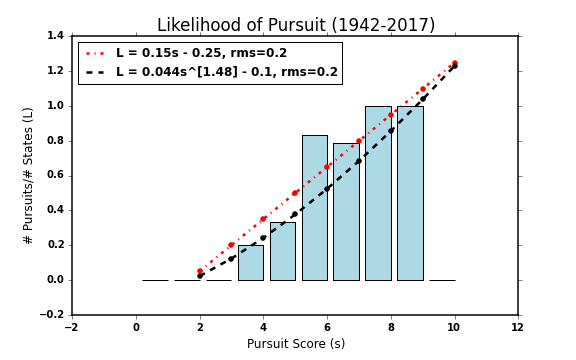
\includegraphics[scale=0.8]{./figs/pe_likely.png}
\end{center}
\caption{Fraction of states with any nuclear technology (dataset from \ref{s_factors}) that pursued weapons at some point in the last 75 years, given their pursuit scores. Although a power-law curve (black) and a weighted linear fit (red) are equivalent with the existing data, a complete set of nation-states would increase the relative weight of lower scores, making the exponential curve a better fit.}
\label{fig:likely}
\end{figure}
 
The score is then converted into a likelihood that the state will pursue a weapon. The relationship between pursuit score and likelihood of pursuing a weapon has been characterized using historical data of the 42 states that have developed nuclear technology since 1942.  \ref{fig:likely} shows the fraction of states with a given pursuit score that pursued a weapon during that time. A power-law (red) or a weighted linear fit (black) are are equivalentl with the 42 state dataset. However, a global dataset of nation-states would have disproportionately lower scores, so we consider the power-law paramaterization to be more representative.


The data shown in \ref{fig:likely} represents the total likelihood integrated over the course of 75 years ($T$). Equation \ref{eqn:likely_eqn} is used to convert to the likelihood of pursuit $L$ in any given year, given a pursuit score $s$.
\begin{equation}
L = 1 - (1 - s)^{1.0/T}
\label{eqn:likely_eqn}
\end{equation}
In the \gls{NWPM} forward model, each state's score is converted to a likelihood of pursuit at that timestep using Equation \ref{eqn:likely_eqn}. The actual conversion is bounded using two heavy-side functions such that scores below a lower threshold (e.g. 4) are forced to a likelihood of zero, while scores above an upper threshold (e.g. 9) are forced to the value of the score at the threshold.   A random number generator is used given the likelihood to determine whether or not the pursuit event occurs. If the determination is for pursuit to occur, the state deploys a secret enrichment facility. If a state is already pursuing a weapon, then the model determines whether it succeeds in acquiring a weapon at that timestep using a median time to acquire of 7.5 years, based on historical data for states that have acquired weapons. On the timestep in which a state succeeds in acquiring a weapon, highly enriched uranium is shipped out of the secret enrichment facility.

\subsection{Limitations of the Historical Data}
The use of historical data to develop a forward model has several limitations. One set of limitations could be improved with a larger historical dataset.  Historical scores for non-nuclear states have not been calculated. Due to the influence of nuclear technology, a non-nuclear state could theoretically have a maximum pursuit score of 7. Considering that the majority of states that have high potential military spending and major historical conflicts have already been incorporated, this further reduces the potential maximum score to below 5, even if all other factors were maximized.  A large fraction of states in the world are have scores on the order of 1-3.  This large set of missing historical data, heavily weighted to the low score side, would reduce the likelihood of higher-score states from pursuing.  The database could also be improved by collecting historical data for many years around dates of pursuit and acquisition rather than just for a single year. This analysis has identified factors that are correlated to weapons programs but there is insufficient data to confirm causal relationships.   

This model is intrinsically limited by the small sample size and the degree to which the global landscape changes over time. With only 10 states that have acquired nuclear weapons throughout history, there is large uncertainty in any quantatitative analysis. Additionally, while conflict has been captured in a crude way, it is difficult to develop a parameterization with enough nuance to capture the varying impact of conflict under paradigms such as World War II, the Cold War, or post-9/11.


\section{Discussion}
\label{s_dis}

The \Cyclus fuel cycle simulator is being used as a framework for combining techniques and knowledge from a variety of disciplines into a cohesive treaty verification approach. This paper presents the diversion of \gls{HEU} as a simple example of measuring facility output as a treaty verification strategy.  This \gls{HEU} simulation used a random-interval, constant-amplitude model to describe the behavior of an illicit actor seeking to divert \gls{HEU} from a declared enrichment facility.  It uses statistical anomaly detection techniques on the data that would be available to an \gls{IAEA} inspector, namely the \gls{LEU} output of the enrichment facility, to demonstrate that material diversion could be detected in this scenario.

This simulation is but one example of the capabilities of \Cyclus as a test bed for treaty verification strategies.  \Cyclus is also being used to model the geographical dissipation of $^{85}Kr$ emission from a covert separations facility processing \gls{WGP} in the effluent shadow of declared facilities.  This feature can be used to assess the required regional distribution of various types of $^{85}Kr$ detectors to ensure detection of clandestine reprocessing programs.  Additionally, \Cyclus has the capability to produce synthetic signals of inherent physical processes such as neutron spectra of various materials.  In this way, \Cyclus simulations can provide theoretical signals to researchers developing experimental detectors in order to test sensitivity and detector response.

Moving forward, \Cyclus will be used to study more complex diversion scenarios.  Probabilistic models for behavior based on risk-perception will be explored.  Ongoing collaborations as part of the \gls{CVT} are examining the mechanisms and limits of expanding anomaly detection algorithms with other types of data, such as social media chatter.  Due to the inherently interdisciplinary nature of this work, new external collaborations are sought with experts in behavioral modeling. Innovative ideas on detection modalities and diversion detection techniques are also welcomed.



\textit{\TODO{This work is funded by the NNSA as part of the Consortium for Verification Technology.  . ..}}
\section{Appendix: Factor Conversion Tables}
\label{s_appendix}

%\iffalse
\begin{table}
\centering
\begin{tabular}{|c|c|c|c|c|c|c|c|c|c|}
\hline
\textbf{Factor Score} & \textbf{Authoritarian} & \textbf{Enrichment}  & \multicolumn{2}{c|}{\textbf{Military Isolation}}    & \textbf{Military Spending} & \textbf{Scientific Network} & \textbf{Nuclear Reactors}  & \textbf{Uranium Reserves} \\
                     &                        &  \textbf{\& Reprocess}& \multicolumn{2}{c|}{$S = 10 - (S_{NNWS} + S_{NWS}$)} & \textbf{(\%GDP)}           &                             &                            &  \\
\cline{4-5}
                    &                         &                        &  $S_{NNWS}$ alliance   & $S_{NWS}$ alliance          &                           &                             &                            & \\


\hline
0                     &  0                     &  0                   &  --                        &  --                     &  --                      &    --                        &      \\   
1                     &  1                     &  --                  &  $<=$ 2                    &  --                     &  $<$ 1                   &    --                        &         \\
2                     &  2                     &  --                  &  (2,4]                     &  --                     &  [1, 2)                  &    --                        &             \\
3                     &  3                     &  --                  &  $> 4$                     &  --                     &  --                      &    --                        &          \\
4                     &  4                     &  --                  &  --                        &  --                     &  [2, 3)                  &     1                        &         \\
5                     &  5                     &  --                  &  --                        &  1                      &  --                      &    --                        &          \\
6                     &  6                     &  --                  &  --                        &  2                      &  --                      &    --                        &          \\
7                     &  7                     &  --                  &  --                        &  $>=$ 3                 &  [3, 5)                  &     2                        &            \\
8                     &  8                     &  --                  &  --                        &  --                     &  --                      &    --                        &           \\
9                     &  9                     &  --                  &  --                        &  --                     &  --                      &    --                        &           \\
10                    &  10                    &  1                   &  --                        &  --                     &   $>=$5                  &     3                        &          \\

\hline
\end{tabular}
\caption{\TODO{CAPTION}}
\label{tab:factor_conversions}
\end{table}


The following scores were defined in a more complex way.

\subsection{Military Isolation}
%Alliances with \gls{NNWS} were assigned a score between 0 and 3, while alliances with \gls{NWS} were assigned a score betwen 5 and 7. These two scores were then summed for the final factor score.


\begin{tabular}{|c|c|c|}
  \hline
   \multicolumn{2}{|c|}{Head 1} & Head 2 \\
  \hline
   a & b & c \\
  \hline
   a & b & c \\
  \hline
\end{tabular}
 


%%%%%%%%%%%%%%%%%%%%%%%%%%%%%%%%%%%%%%%%%%%%%%%%%%%%%%%%%%%%%%%%%%%%%%%%%%%%%%%%
\begin{small}
\bibliographystyle{ANSurl}
\bibliography{../zotero_160516,../zotero_adds_160603,../manual_fixes,../websites_manual}
\end{small}
\end{document}
